\documentclass[11pt, compress, aspectratio=1610, serif]{beamer}

\usetheme{pl}

\usepackage{booktabs}
\usepackage{minted}
\usepackage{listings}
\usepackage{color}
\usepackage{fancyvrb}
\newcommand{\VerbBar}{|}
\newcommand{\VERB}{\Verb[commandchars=\\\{\}]}
\DefineVerbatimEnvironment{Highlighting}{Verbatim}{commandchars=\\\{\}}
% Add ',fontsize=\small' for more characters per line
\newenvironment{Shaded}{}{}
\newcommand{\KeywordTok}[1]{\textcolor[rgb]{0.00,0.44,0.13}{\textbf{{#1}}}}
\newcommand{\DataTypeTok}[1]{\textcolor[rgb]{0.56,0.13,0.00}{{#1}}}
\newcommand{\DecValTok}[1]{\textcolor[rgb]{0.25,0.63,0.44}{{#1}}}
\newcommand{\BaseNTok}[1]{\textcolor[rgb]{0.25,0.63,0.44}{{#1}}}
\newcommand{\FloatTok}[1]{\textcolor[rgb]{0.25,0.63,0.44}{{#1}}}
\newcommand{\ConstantTok}[1]{\textcolor[rgb]{0.53,0.00,0.00}{{#1}}}
\newcommand{\CharTok}[1]{\textcolor[rgb]{0.25,0.44,0.63}{{#1}}}
\newcommand{\SpecialCharTok}[1]{\textcolor[rgb]{0.25,0.44,0.63}{{#1}}}
\newcommand{\StringTok}[1]{\textcolor[rgb]{0.25,0.44,0.63}{{#1}}}
\newcommand{\VerbatimStringTok}[1]{\textcolor[rgb]{0.25,0.44,0.63}{{#1}}}
\newcommand{\SpecialStringTok}[1]{\textcolor[rgb]{0.73,0.40,0.53}{{#1}}}
\newcommand{\ImportTok}[1]{{#1}}
\newcommand{\CommentTok}[1]{\textcolor[rgb]{0.38,0.63,0.69}{\textit{{#1}}}}
\newcommand{\DocumentationTok}[1]{\textcolor[rgb]{0.73,0.13,0.13}{\textit{{#1}}}}
\newcommand{\AnnotationTok}[1]{\textcolor[rgb]{0.38,0.63,0.69}{\textbf{\textit{{#1}}}}}
\newcommand{\CommentVarTok}[1]{\textcolor[rgb]{0.38,0.63,0.69}{\textbf{\textit{{#1}}}}}
\newcommand{\OtherTok}[1]{\textcolor[rgb]{0.00,0.44,0.13}{{#1}}}
\newcommand{\FunctionTok}[1]{\textcolor[rgb]{0.02,0.16,0.49}{{#1}}}
\newcommand{\VariableTok}[1]{\textcolor[rgb]{0.10,0.09,0.49}{{#1}}}
\newcommand{\ControlFlowTok}[1]{\textcolor[rgb]{0.00,0.44,0.13}{\textbf{{#1}}}}
\newcommand{\OperatorTok}[1]{\textcolor[rgb]{0.40,0.40,0.40}{{#1}}}
\newcommand{\BuiltInTok}[1]{{#1}}
\newcommand{\ExtensionTok}[1]{{#1}}
\newcommand{\PreprocessorTok}[1]{\textcolor[rgb]{0.74,0.48,0.00}{{#1}}}
\newcommand{\AttributeTok}[1]{\textcolor[rgb]{0.49,0.56,0.16}{{#1}}}
\newcommand{\RegionMarkerTok}[1]{{#1}}
\newcommand{\InformationTok}[1]{\textcolor[rgb]{0.38,0.63,0.69}{\textbf{\textit{{#1}}}}}
\newcommand{\WarningTok}[1]{\textcolor[rgb]{0.38,0.63,0.69}{\textbf{\textit{{#1}}}}}
\newcommand{\AlertTok}[1]{\textcolor[rgb]{1.00,0.00,0.00}{\textbf{{#1}}}}
\newcommand{\ErrorTok}[1]{\textcolor[rgb]{1.00,0.00,0.00}{\textbf{{#1}}}}
\newcommand{\NormalTok}[1]{{#1}}

\makeatletter
\def\maxwidth{\ifdim\Gin@nat@width>\linewidth\linewidth\else\Gin@nat@width\fi}
\makeatother

\usepgfplotslibrary{dateplot}

\newcommand{\begincols}{\begin{columns}}
\newcommand{\stopcols}{\end{columns}}

\title{EcologicalNetwork.jl}
\subtitle{Analysis of ecological interactions}
\date{\today}
\author{Timothée Poisot}
\institute{Université de Montréal}

\begin{document}

\maketitle

\begin{frame}[fragile]{The \texttt{EcologicalNetwork} package}

\begin{Shaded}
\begin{Highlighting}[]
\NormalTok{using EcologicalNetwork}
\NormalTok{data = ollerton();}

\NormalTok{η(data)}
\end{Highlighting}
\end{Shaded}

\begin{verbatim}
3-element Array{Float64,1}:
 0.640955
 0.646288
 0.635621
\end{verbatim}

\end{frame}

\section{Visualising networks}\label{visualising-networks}

\begin{frame}[fragile]{Setting up the environment}

\begin{Shaded}
\begin{Highlighting}[]
\NormalTok{using Plots}
\NormalTok{pgfplots()}
\end{Highlighting}
\end{Shaded}

\begin{verbatim}
Plots.PGFPlotsBackend()
\end{verbatim}

\end{frame}

\begin{frame}[fragile]{Default plotting}

\begincols
\column{0.48\textwidth}

\begin{Shaded}
\begin{Highlighting}[]
\NormalTok{p1 = plot(data, size=(}\FloatTok{250}\NormalTok{, }\FloatTok{100}\NormalTok{));}
\NormalTok{savefig(p1, }\StringTok{"figures/ollerton.tex"}\NormalTok{);}
\end{Highlighting}
\end{Shaded}

\hfill\column{0.48\textwidth}

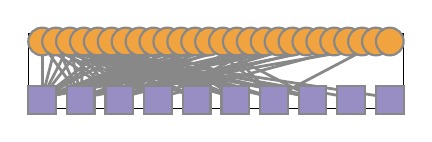
\begin{tikzpicture}[]
\begin{axis}[height = {25.4mm}, ylabel = {}, xmin = {0}, xmax = {27}, ymax = {8}, xlabel = {}, {unbounded coords=jump, xticklabel style={rotate = 0}, xmajorticks=false, yticklabel style={rotate = 0}, ymajorticks=false,     xshift = 0.0mm,
    yshift = 0.0mm,
    axis background/.style={fill={rgb,1:red,1.00000000;green,1.00000000;blue,1.00000000}}
}, ymin = {-1}, width = {63.5mm}]\addplot+ [color = {rgb,1:red,0.53333333;green,0.53333333;blue,0.53333333},
draw opacity=1.0,
line width=1,
solid,mark = none,
mark size = 5.0,
mark options = {
    color = {rgb,1:red,0.53333333;green,0.53333333;blue,0.53333333}, draw opacity = 1.0,
    fill = {rgb,1:red,0.53333333;green,0.53333333;blue,0.53333333}, fill opacity = 1.0,
    line width = 0.8,
    rotate = 0,
    solid
},forget plot]coordinates {
(1.0, 6.7)
(1.0, 0.3)
};
\addplot+ [color = {rgb,1:red,0.53333333;green,0.53333333;blue,0.53333333},
draw opacity=1.0,
line width=1,
solid,mark = none,
mark size = 5.0,
mark options = {
    color = {rgb,1:red,0.53333333;green,0.53333333;blue,0.53333333}, draw opacity = 1.0,
    fill = {rgb,1:red,0.53333333;green,0.53333333;blue,0.53333333}, fill opacity = 1.0,
    line width = 0.8,
    rotate = 0,
    solid
},forget plot]coordinates {
(1.0, 6.7)
(3.7777777777777777, 0.3)
};
\addplot+ [color = {rgb,1:red,0.53333333;green,0.53333333;blue,0.53333333},
draw opacity=1.0,
line width=1,
solid,mark = none,
mark size = 5.0,
mark options = {
    color = {rgb,1:red,0.53333333;green,0.53333333;blue,0.53333333}, draw opacity = 1.0,
    fill = {rgb,1:red,0.53333333;green,0.53333333;blue,0.53333333}, fill opacity = 1.0,
    line width = 0.8,
    rotate = 0,
    solid
},forget plot]coordinates {
(1.0, 6.7)
(6.555555555555555, 0.3)
};
\addplot+ [color = {rgb,1:red,0.53333333;green,0.53333333;blue,0.53333333},
draw opacity=1.0,
line width=1,
solid,mark = none,
mark size = 5.0,
mark options = {
    color = {rgb,1:red,0.53333333;green,0.53333333;blue,0.53333333}, draw opacity = 1.0,
    fill = {rgb,1:red,0.53333333;green,0.53333333;blue,0.53333333}, fill opacity = 1.0,
    line width = 0.8,
    rotate = 0,
    solid
},forget plot]coordinates {
(1.0, 6.7)
(9.333333333333334, 0.3)
};
\addplot+ [color = {rgb,1:red,0.53333333;green,0.53333333;blue,0.53333333},
draw opacity=1.0,
line width=1,
solid,mark = none,
mark size = 5.0,
mark options = {
    color = {rgb,1:red,0.53333333;green,0.53333333;blue,0.53333333}, draw opacity = 1.0,
    fill = {rgb,1:red,0.53333333;green,0.53333333;blue,0.53333333}, fill opacity = 1.0,
    line width = 0.8,
    rotate = 0,
    solid
},forget plot]coordinates {
(1.0, 6.7)
(12.11111111111111, 0.3)
};
\addplot+ [color = {rgb,1:red,0.53333333;green,0.53333333;blue,0.53333333},
draw opacity=1.0,
line width=1,
solid,mark = none,
mark size = 5.0,
mark options = {
    color = {rgb,1:red,0.53333333;green,0.53333333;blue,0.53333333}, draw opacity = 1.0,
    fill = {rgb,1:red,0.53333333;green,0.53333333;blue,0.53333333}, fill opacity = 1.0,
    line width = 0.8,
    rotate = 0,
    solid
},forget plot]coordinates {
(1.0, 6.7)
(14.88888888888889, 0.3)
};
\addplot+ [color = {rgb,1:red,0.53333333;green,0.53333333;blue,0.53333333},
draw opacity=1.0,
line width=1,
solid,mark = none,
mark size = 5.0,
mark options = {
    color = {rgb,1:red,0.53333333;green,0.53333333;blue,0.53333333}, draw opacity = 1.0,
    fill = {rgb,1:red,0.53333333;green,0.53333333;blue,0.53333333}, fill opacity = 1.0,
    line width = 0.8,
    rotate = 0,
    solid
},forget plot]coordinates {
(1.0, 6.7)
(17.666666666666668, 0.3)
};
\addplot+ [color = {rgb,1:red,0.53333333;green,0.53333333;blue,0.53333333},
draw opacity=1.0,
line width=1,
solid,mark = none,
mark size = 5.0,
mark options = {
    color = {rgb,1:red,0.53333333;green,0.53333333;blue,0.53333333}, draw opacity = 1.0,
    fill = {rgb,1:red,0.53333333;green,0.53333333;blue,0.53333333}, fill opacity = 1.0,
    line width = 0.8,
    rotate = 0,
    solid
},forget plot]coordinates {
(1.0, 6.7)
(20.444444444444443, 0.3)
};
\addplot+ [color = {rgb,1:red,0.53333333;green,0.53333333;blue,0.53333333},
draw opacity=1.0,
line width=1,
solid,mark = none,
mark size = 5.0,
mark options = {
    color = {rgb,1:red,0.53333333;green,0.53333333;blue,0.53333333}, draw opacity = 1.0,
    fill = {rgb,1:red,0.53333333;green,0.53333333;blue,0.53333333}, fill opacity = 1.0,
    line width = 0.8,
    rotate = 0,
    solid
},forget plot]coordinates {
(1.0, 6.7)
(23.22222222222222, 0.3)
};
\addplot+ [color = {rgb,1:red,0.53333333;green,0.53333333;blue,0.53333333},
draw opacity=1.0,
line width=1,
solid,mark = none,
mark size = 5.0,
mark options = {
    color = {rgb,1:red,0.53333333;green,0.53333333;blue,0.53333333}, draw opacity = 1.0,
    fill = {rgb,1:red,0.53333333;green,0.53333333;blue,0.53333333}, fill opacity = 1.0,
    line width = 0.8,
    rotate = 0,
    solid
},forget plot]coordinates {
(1.0, 6.7)
(26.0, 0.3)
};
\addplot+ [color = {rgb,1:red,0.53333333;green,0.53333333;blue,0.53333333},
draw opacity=1.0,
line width=1,
solid,mark = none,
mark size = 5.0,
mark options = {
    color = {rgb,1:red,0.53333333;green,0.53333333;blue,0.53333333}, draw opacity = 1.0,
    fill = {rgb,1:red,0.53333333;green,0.53333333;blue,0.53333333}, fill opacity = 1.0,
    line width = 0.8,
    rotate = 0,
    solid
},forget plot]coordinates {
(2.0, 6.7)
(1.0, 0.3)
};
\addplot+ [color = {rgb,1:red,0.53333333;green,0.53333333;blue,0.53333333},
draw opacity=1.0,
line width=1,
solid,mark = none,
mark size = 5.0,
mark options = {
    color = {rgb,1:red,0.53333333;green,0.53333333;blue,0.53333333}, draw opacity = 1.0,
    fill = {rgb,1:red,0.53333333;green,0.53333333;blue,0.53333333}, fill opacity = 1.0,
    line width = 0.8,
    rotate = 0,
    solid
},forget plot]coordinates {
(2.0, 6.7)
(3.7777777777777777, 0.3)
};
\addplot+ [color = {rgb,1:red,0.53333333;green,0.53333333;blue,0.53333333},
draw opacity=1.0,
line width=1,
solid,mark = none,
mark size = 5.0,
mark options = {
    color = {rgb,1:red,0.53333333;green,0.53333333;blue,0.53333333}, draw opacity = 1.0,
    fill = {rgb,1:red,0.53333333;green,0.53333333;blue,0.53333333}, fill opacity = 1.0,
    line width = 0.8,
    rotate = 0,
    solid
},forget plot]coordinates {
(2.0, 6.7)
(6.555555555555555, 0.3)
};
\addplot+ [color = {rgb,1:red,0.53333333;green,0.53333333;blue,0.53333333},
draw opacity=1.0,
line width=1,
solid,mark = none,
mark size = 5.0,
mark options = {
    color = {rgb,1:red,0.53333333;green,0.53333333;blue,0.53333333}, draw opacity = 1.0,
    fill = {rgb,1:red,0.53333333;green,0.53333333;blue,0.53333333}, fill opacity = 1.0,
    line width = 0.8,
    rotate = 0,
    solid
},forget plot]coordinates {
(2.0, 6.7)
(9.333333333333334, 0.3)
};
\addplot+ [color = {rgb,1:red,0.53333333;green,0.53333333;blue,0.53333333},
draw opacity=1.0,
line width=1,
solid,mark = none,
mark size = 5.0,
mark options = {
    color = {rgb,1:red,0.53333333;green,0.53333333;blue,0.53333333}, draw opacity = 1.0,
    fill = {rgb,1:red,0.53333333;green,0.53333333;blue,0.53333333}, fill opacity = 1.0,
    line width = 0.8,
    rotate = 0,
    solid
},forget plot]coordinates {
(2.0, 6.7)
(12.11111111111111, 0.3)
};
\addplot+ [color = {rgb,1:red,0.53333333;green,0.53333333;blue,0.53333333},
draw opacity=1.0,
line width=1,
solid,mark = none,
mark size = 5.0,
mark options = {
    color = {rgb,1:red,0.53333333;green,0.53333333;blue,0.53333333}, draw opacity = 1.0,
    fill = {rgb,1:red,0.53333333;green,0.53333333;blue,0.53333333}, fill opacity = 1.0,
    line width = 0.8,
    rotate = 0,
    solid
},forget plot]coordinates {
(2.0, 6.7)
(14.88888888888889, 0.3)
};
\addplot+ [color = {rgb,1:red,0.53333333;green,0.53333333;blue,0.53333333},
draw opacity=1.0,
line width=1,
solid,mark = none,
mark size = 5.0,
mark options = {
    color = {rgb,1:red,0.53333333;green,0.53333333;blue,0.53333333}, draw opacity = 1.0,
    fill = {rgb,1:red,0.53333333;green,0.53333333;blue,0.53333333}, fill opacity = 1.0,
    line width = 0.8,
    rotate = 0,
    solid
},forget plot]coordinates {
(2.0, 6.7)
(17.666666666666668, 0.3)
};
\addplot+ [color = {rgb,1:red,0.53333333;green,0.53333333;blue,0.53333333},
draw opacity=1.0,
line width=1,
solid,mark = none,
mark size = 5.0,
mark options = {
    color = {rgb,1:red,0.53333333;green,0.53333333;blue,0.53333333}, draw opacity = 1.0,
    fill = {rgb,1:red,0.53333333;green,0.53333333;blue,0.53333333}, fill opacity = 1.0,
    line width = 0.8,
    rotate = 0,
    solid
},forget plot]coordinates {
(3.0, 6.7)
(1.0, 0.3)
};
\addplot+ [color = {rgb,1:red,0.53333333;green,0.53333333;blue,0.53333333},
draw opacity=1.0,
line width=1,
solid,mark = none,
mark size = 5.0,
mark options = {
    color = {rgb,1:red,0.53333333;green,0.53333333;blue,0.53333333}, draw opacity = 1.0,
    fill = {rgb,1:red,0.53333333;green,0.53333333;blue,0.53333333}, fill opacity = 1.0,
    line width = 0.8,
    rotate = 0,
    solid
},forget plot]coordinates {
(3.0, 6.7)
(3.7777777777777777, 0.3)
};
\addplot+ [color = {rgb,1:red,0.53333333;green,0.53333333;blue,0.53333333},
draw opacity=1.0,
line width=1,
solid,mark = none,
mark size = 5.0,
mark options = {
    color = {rgb,1:red,0.53333333;green,0.53333333;blue,0.53333333}, draw opacity = 1.0,
    fill = {rgb,1:red,0.53333333;green,0.53333333;blue,0.53333333}, fill opacity = 1.0,
    line width = 0.8,
    rotate = 0,
    solid
},forget plot]coordinates {
(3.0, 6.7)
(6.555555555555555, 0.3)
};
\addplot+ [color = {rgb,1:red,0.53333333;green,0.53333333;blue,0.53333333},
draw opacity=1.0,
line width=1,
solid,mark = none,
mark size = 5.0,
mark options = {
    color = {rgb,1:red,0.53333333;green,0.53333333;blue,0.53333333}, draw opacity = 1.0,
    fill = {rgb,1:red,0.53333333;green,0.53333333;blue,0.53333333}, fill opacity = 1.0,
    line width = 0.8,
    rotate = 0,
    solid
},forget plot]coordinates {
(3.0, 6.7)
(9.333333333333334, 0.3)
};
\addplot+ [color = {rgb,1:red,0.53333333;green,0.53333333;blue,0.53333333},
draw opacity=1.0,
line width=1,
solid,mark = none,
mark size = 5.0,
mark options = {
    color = {rgb,1:red,0.53333333;green,0.53333333;blue,0.53333333}, draw opacity = 1.0,
    fill = {rgb,1:red,0.53333333;green,0.53333333;blue,0.53333333}, fill opacity = 1.0,
    line width = 0.8,
    rotate = 0,
    solid
},forget plot]coordinates {
(3.0, 6.7)
(14.88888888888889, 0.3)
};
\addplot+ [color = {rgb,1:red,0.53333333;green,0.53333333;blue,0.53333333},
draw opacity=1.0,
line width=1,
solid,mark = none,
mark size = 5.0,
mark options = {
    color = {rgb,1:red,0.53333333;green,0.53333333;blue,0.53333333}, draw opacity = 1.0,
    fill = {rgb,1:red,0.53333333;green,0.53333333;blue,0.53333333}, fill opacity = 1.0,
    line width = 0.8,
    rotate = 0,
    solid
},forget plot]coordinates {
(3.0, 6.7)
(17.666666666666668, 0.3)
};
\addplot+ [color = {rgb,1:red,0.53333333;green,0.53333333;blue,0.53333333},
draw opacity=1.0,
line width=1,
solid,mark = none,
mark size = 5.0,
mark options = {
    color = {rgb,1:red,0.53333333;green,0.53333333;blue,0.53333333}, draw opacity = 1.0,
    fill = {rgb,1:red,0.53333333;green,0.53333333;blue,0.53333333}, fill opacity = 1.0,
    line width = 0.8,
    rotate = 0,
    solid
},forget plot]coordinates {
(3.0, 6.7)
(20.444444444444443, 0.3)
};
\addplot+ [color = {rgb,1:red,0.53333333;green,0.53333333;blue,0.53333333},
draw opacity=1.0,
line width=1,
solid,mark = none,
mark size = 5.0,
mark options = {
    color = {rgb,1:red,0.53333333;green,0.53333333;blue,0.53333333}, draw opacity = 1.0,
    fill = {rgb,1:red,0.53333333;green,0.53333333;blue,0.53333333}, fill opacity = 1.0,
    line width = 0.8,
    rotate = 0,
    solid
},forget plot]coordinates {
(4.0, 6.7)
(1.0, 0.3)
};
\addplot+ [color = {rgb,1:red,0.53333333;green,0.53333333;blue,0.53333333},
draw opacity=1.0,
line width=1,
solid,mark = none,
mark size = 5.0,
mark options = {
    color = {rgb,1:red,0.53333333;green,0.53333333;blue,0.53333333}, draw opacity = 1.0,
    fill = {rgb,1:red,0.53333333;green,0.53333333;blue,0.53333333}, fill opacity = 1.0,
    line width = 0.8,
    rotate = 0,
    solid
},forget plot]coordinates {
(4.0, 6.7)
(3.7777777777777777, 0.3)
};
\addplot+ [color = {rgb,1:red,0.53333333;green,0.53333333;blue,0.53333333},
draw opacity=1.0,
line width=1,
solid,mark = none,
mark size = 5.0,
mark options = {
    color = {rgb,1:red,0.53333333;green,0.53333333;blue,0.53333333}, draw opacity = 1.0,
    fill = {rgb,1:red,0.53333333;green,0.53333333;blue,0.53333333}, fill opacity = 1.0,
    line width = 0.8,
    rotate = 0,
    solid
},forget plot]coordinates {
(4.0, 6.7)
(6.555555555555555, 0.3)
};
\addplot+ [color = {rgb,1:red,0.53333333;green,0.53333333;blue,0.53333333},
draw opacity=1.0,
line width=1,
solid,mark = none,
mark size = 5.0,
mark options = {
    color = {rgb,1:red,0.53333333;green,0.53333333;blue,0.53333333}, draw opacity = 1.0,
    fill = {rgb,1:red,0.53333333;green,0.53333333;blue,0.53333333}, fill opacity = 1.0,
    line width = 0.8,
    rotate = 0,
    solid
},forget plot]coordinates {
(4.0, 6.7)
(9.333333333333334, 0.3)
};
\addplot+ [color = {rgb,1:red,0.53333333;green,0.53333333;blue,0.53333333},
draw opacity=1.0,
line width=1,
solid,mark = none,
mark size = 5.0,
mark options = {
    color = {rgb,1:red,0.53333333;green,0.53333333;blue,0.53333333}, draw opacity = 1.0,
    fill = {rgb,1:red,0.53333333;green,0.53333333;blue,0.53333333}, fill opacity = 1.0,
    line width = 0.8,
    rotate = 0,
    solid
},forget plot]coordinates {
(4.0, 6.7)
(12.11111111111111, 0.3)
};
\addplot+ [color = {rgb,1:red,0.53333333;green,0.53333333;blue,0.53333333},
draw opacity=1.0,
line width=1,
solid,mark = none,
mark size = 5.0,
mark options = {
    color = {rgb,1:red,0.53333333;green,0.53333333;blue,0.53333333}, draw opacity = 1.0,
    fill = {rgb,1:red,0.53333333;green,0.53333333;blue,0.53333333}, fill opacity = 1.0,
    line width = 0.8,
    rotate = 0,
    solid
},forget plot]coordinates {
(4.0, 6.7)
(14.88888888888889, 0.3)
};
\addplot+ [color = {rgb,1:red,0.53333333;green,0.53333333;blue,0.53333333},
draw opacity=1.0,
line width=1,
solid,mark = none,
mark size = 5.0,
mark options = {
    color = {rgb,1:red,0.53333333;green,0.53333333;blue,0.53333333}, draw opacity = 1.0,
    fill = {rgb,1:red,0.53333333;green,0.53333333;blue,0.53333333}, fill opacity = 1.0,
    line width = 0.8,
    rotate = 0,
    solid
},forget plot]coordinates {
(5.0, 6.7)
(6.555555555555555, 0.3)
};
\addplot+ [color = {rgb,1:red,0.53333333;green,0.53333333;blue,0.53333333},
draw opacity=1.0,
line width=1,
solid,mark = none,
mark size = 5.0,
mark options = {
    color = {rgb,1:red,0.53333333;green,0.53333333;blue,0.53333333}, draw opacity = 1.0,
    fill = {rgb,1:red,0.53333333;green,0.53333333;blue,0.53333333}, fill opacity = 1.0,
    line width = 0.8,
    rotate = 0,
    solid
},forget plot]coordinates {
(5.0, 6.7)
(9.333333333333334, 0.3)
};
\addplot+ [color = {rgb,1:red,0.53333333;green,0.53333333;blue,0.53333333},
draw opacity=1.0,
line width=1,
solid,mark = none,
mark size = 5.0,
mark options = {
    color = {rgb,1:red,0.53333333;green,0.53333333;blue,0.53333333}, draw opacity = 1.0,
    fill = {rgb,1:red,0.53333333;green,0.53333333;blue,0.53333333}, fill opacity = 1.0,
    line width = 0.8,
    rotate = 0,
    solid
},forget plot]coordinates {
(5.0, 6.7)
(14.88888888888889, 0.3)
};
\addplot+ [color = {rgb,1:red,0.53333333;green,0.53333333;blue,0.53333333},
draw opacity=1.0,
line width=1,
solid,mark = none,
mark size = 5.0,
mark options = {
    color = {rgb,1:red,0.53333333;green,0.53333333;blue,0.53333333}, draw opacity = 1.0,
    fill = {rgb,1:red,0.53333333;green,0.53333333;blue,0.53333333}, fill opacity = 1.0,
    line width = 0.8,
    rotate = 0,
    solid
},forget plot]coordinates {
(5.0, 6.7)
(17.666666666666668, 0.3)
};
\addplot+ [color = {rgb,1:red,0.53333333;green,0.53333333;blue,0.53333333},
draw opacity=1.0,
line width=1,
solid,mark = none,
mark size = 5.0,
mark options = {
    color = {rgb,1:red,0.53333333;green,0.53333333;blue,0.53333333}, draw opacity = 1.0,
    fill = {rgb,1:red,0.53333333;green,0.53333333;blue,0.53333333}, fill opacity = 1.0,
    line width = 0.8,
    rotate = 0,
    solid
},forget plot]coordinates {
(6.0, 6.7)
(1.0, 0.3)
};
\addplot+ [color = {rgb,1:red,0.53333333;green,0.53333333;blue,0.53333333},
draw opacity=1.0,
line width=1,
solid,mark = none,
mark size = 5.0,
mark options = {
    color = {rgb,1:red,0.53333333;green,0.53333333;blue,0.53333333}, draw opacity = 1.0,
    fill = {rgb,1:red,0.53333333;green,0.53333333;blue,0.53333333}, fill opacity = 1.0,
    line width = 0.8,
    rotate = 0,
    solid
},forget plot]coordinates {
(6.0, 6.7)
(3.7777777777777777, 0.3)
};
\addplot+ [color = {rgb,1:red,0.53333333;green,0.53333333;blue,0.53333333},
draw opacity=1.0,
line width=1,
solid,mark = none,
mark size = 5.0,
mark options = {
    color = {rgb,1:red,0.53333333;green,0.53333333;blue,0.53333333}, draw opacity = 1.0,
    fill = {rgb,1:red,0.53333333;green,0.53333333;blue,0.53333333}, fill opacity = 1.0,
    line width = 0.8,
    rotate = 0,
    solid
},forget plot]coordinates {
(6.0, 6.7)
(6.555555555555555, 0.3)
};
\addplot+ [color = {rgb,1:red,0.53333333;green,0.53333333;blue,0.53333333},
draw opacity=1.0,
line width=1,
solid,mark = none,
mark size = 5.0,
mark options = {
    color = {rgb,1:red,0.53333333;green,0.53333333;blue,0.53333333}, draw opacity = 1.0,
    fill = {rgb,1:red,0.53333333;green,0.53333333;blue,0.53333333}, fill opacity = 1.0,
    line width = 0.8,
    rotate = 0,
    solid
},forget plot]coordinates {
(6.0, 6.7)
(14.88888888888889, 0.3)
};
\addplot+ [color = {rgb,1:red,0.53333333;green,0.53333333;blue,0.53333333},
draw opacity=1.0,
line width=1,
solid,mark = none,
mark size = 5.0,
mark options = {
    color = {rgb,1:red,0.53333333;green,0.53333333;blue,0.53333333}, draw opacity = 1.0,
    fill = {rgb,1:red,0.53333333;green,0.53333333;blue,0.53333333}, fill opacity = 1.0,
    line width = 0.8,
    rotate = 0,
    solid
},forget plot]coordinates {
(7.0, 6.7)
(1.0, 0.3)
};
\addplot+ [color = {rgb,1:red,0.53333333;green,0.53333333;blue,0.53333333},
draw opacity=1.0,
line width=1,
solid,mark = none,
mark size = 5.0,
mark options = {
    color = {rgb,1:red,0.53333333;green,0.53333333;blue,0.53333333}, draw opacity = 1.0,
    fill = {rgb,1:red,0.53333333;green,0.53333333;blue,0.53333333}, fill opacity = 1.0,
    line width = 0.8,
    rotate = 0,
    solid
},forget plot]coordinates {
(7.0, 6.7)
(9.333333333333334, 0.3)
};
\addplot+ [color = {rgb,1:red,0.53333333;green,0.53333333;blue,0.53333333},
draw opacity=1.0,
line width=1,
solid,mark = none,
mark size = 5.0,
mark options = {
    color = {rgb,1:red,0.53333333;green,0.53333333;blue,0.53333333}, draw opacity = 1.0,
    fill = {rgb,1:red,0.53333333;green,0.53333333;blue,0.53333333}, fill opacity = 1.0,
    line width = 0.8,
    rotate = 0,
    solid
},forget plot]coordinates {
(7.0, 6.7)
(12.11111111111111, 0.3)
};
\addplot+ [color = {rgb,1:red,0.53333333;green,0.53333333;blue,0.53333333},
draw opacity=1.0,
line width=1,
solid,mark = none,
mark size = 5.0,
mark options = {
    color = {rgb,1:red,0.53333333;green,0.53333333;blue,0.53333333}, draw opacity = 1.0,
    fill = {rgb,1:red,0.53333333;green,0.53333333;blue,0.53333333}, fill opacity = 1.0,
    line width = 0.8,
    rotate = 0,
    solid
},forget plot]coordinates {
(7.0, 6.7)
(20.444444444444443, 0.3)
};
\addplot+ [color = {rgb,1:red,0.53333333;green,0.53333333;blue,0.53333333},
draw opacity=1.0,
line width=1,
solid,mark = none,
mark size = 5.0,
mark options = {
    color = {rgb,1:red,0.53333333;green,0.53333333;blue,0.53333333}, draw opacity = 1.0,
    fill = {rgb,1:red,0.53333333;green,0.53333333;blue,0.53333333}, fill opacity = 1.0,
    line width = 0.8,
    rotate = 0,
    solid
},forget plot]coordinates {
(8.0, 6.7)
(1.0, 0.3)
};
\addplot+ [color = {rgb,1:red,0.53333333;green,0.53333333;blue,0.53333333},
draw opacity=1.0,
line width=1,
solid,mark = none,
mark size = 5.0,
mark options = {
    color = {rgb,1:red,0.53333333;green,0.53333333;blue,0.53333333}, draw opacity = 1.0,
    fill = {rgb,1:red,0.53333333;green,0.53333333;blue,0.53333333}, fill opacity = 1.0,
    line width = 0.8,
    rotate = 0,
    solid
},forget plot]coordinates {
(8.0, 6.7)
(3.7777777777777777, 0.3)
};
\addplot+ [color = {rgb,1:red,0.53333333;green,0.53333333;blue,0.53333333},
draw opacity=1.0,
line width=1,
solid,mark = none,
mark size = 5.0,
mark options = {
    color = {rgb,1:red,0.53333333;green,0.53333333;blue,0.53333333}, draw opacity = 1.0,
    fill = {rgb,1:red,0.53333333;green,0.53333333;blue,0.53333333}, fill opacity = 1.0,
    line width = 0.8,
    rotate = 0,
    solid
},forget plot]coordinates {
(8.0, 6.7)
(9.333333333333334, 0.3)
};
\addplot+ [color = {rgb,1:red,0.53333333;green,0.53333333;blue,0.53333333},
draw opacity=1.0,
line width=1,
solid,mark = none,
mark size = 5.0,
mark options = {
    color = {rgb,1:red,0.53333333;green,0.53333333;blue,0.53333333}, draw opacity = 1.0,
    fill = {rgb,1:red,0.53333333;green,0.53333333;blue,0.53333333}, fill opacity = 1.0,
    line width = 0.8,
    rotate = 0,
    solid
},forget plot]coordinates {
(8.0, 6.7)
(12.11111111111111, 0.3)
};
\addplot+ [color = {rgb,1:red,0.53333333;green,0.53333333;blue,0.53333333},
draw opacity=1.0,
line width=1,
solid,mark = none,
mark size = 5.0,
mark options = {
    color = {rgb,1:red,0.53333333;green,0.53333333;blue,0.53333333}, draw opacity = 1.0,
    fill = {rgb,1:red,0.53333333;green,0.53333333;blue,0.53333333}, fill opacity = 1.0,
    line width = 0.8,
    rotate = 0,
    solid
},forget plot]coordinates {
(9.0, 6.7)
(3.7777777777777777, 0.3)
};
\addplot+ [color = {rgb,1:red,0.53333333;green,0.53333333;blue,0.53333333},
draw opacity=1.0,
line width=1,
solid,mark = none,
mark size = 5.0,
mark options = {
    color = {rgb,1:red,0.53333333;green,0.53333333;blue,0.53333333}, draw opacity = 1.0,
    fill = {rgb,1:red,0.53333333;green,0.53333333;blue,0.53333333}, fill opacity = 1.0,
    line width = 0.8,
    rotate = 0,
    solid
},forget plot]coordinates {
(9.0, 6.7)
(6.555555555555555, 0.3)
};
\addplot+ [color = {rgb,1:red,0.53333333;green,0.53333333;blue,0.53333333},
draw opacity=1.0,
line width=1,
solid,mark = none,
mark size = 5.0,
mark options = {
    color = {rgb,1:red,0.53333333;green,0.53333333;blue,0.53333333}, draw opacity = 1.0,
    fill = {rgb,1:red,0.53333333;green,0.53333333;blue,0.53333333}, fill opacity = 1.0,
    line width = 0.8,
    rotate = 0,
    solid
},forget plot]coordinates {
(9.0, 6.7)
(14.88888888888889, 0.3)
};
\addplot+ [color = {rgb,1:red,0.53333333;green,0.53333333;blue,0.53333333},
draw opacity=1.0,
line width=1,
solid,mark = none,
mark size = 5.0,
mark options = {
    color = {rgb,1:red,0.53333333;green,0.53333333;blue,0.53333333}, draw opacity = 1.0,
    fill = {rgb,1:red,0.53333333;green,0.53333333;blue,0.53333333}, fill opacity = 1.0,
    line width = 0.8,
    rotate = 0,
    solid
},forget plot]coordinates {
(10.0, 6.7)
(6.555555555555555, 0.3)
};
\addplot+ [color = {rgb,1:red,0.53333333;green,0.53333333;blue,0.53333333},
draw opacity=1.0,
line width=1,
solid,mark = none,
mark size = 5.0,
mark options = {
    color = {rgb,1:red,0.53333333;green,0.53333333;blue,0.53333333}, draw opacity = 1.0,
    fill = {rgb,1:red,0.53333333;green,0.53333333;blue,0.53333333}, fill opacity = 1.0,
    line width = 0.8,
    rotate = 0,
    solid
},forget plot]coordinates {
(10.0, 6.7)
(9.333333333333334, 0.3)
};
\addplot+ [color = {rgb,1:red,0.53333333;green,0.53333333;blue,0.53333333},
draw opacity=1.0,
line width=1,
solid,mark = none,
mark size = 5.0,
mark options = {
    color = {rgb,1:red,0.53333333;green,0.53333333;blue,0.53333333}, draw opacity = 1.0,
    fill = {rgb,1:red,0.53333333;green,0.53333333;blue,0.53333333}, fill opacity = 1.0,
    line width = 0.8,
    rotate = 0,
    solid
},forget plot]coordinates {
(10.0, 6.7)
(12.11111111111111, 0.3)
};
\addplot+ [color = {rgb,1:red,0.53333333;green,0.53333333;blue,0.53333333},
draw opacity=1.0,
line width=1,
solid,mark = none,
mark size = 5.0,
mark options = {
    color = {rgb,1:red,0.53333333;green,0.53333333;blue,0.53333333}, draw opacity = 1.0,
    fill = {rgb,1:red,0.53333333;green,0.53333333;blue,0.53333333}, fill opacity = 1.0,
    line width = 0.8,
    rotate = 0,
    solid
},forget plot]coordinates {
(11.0, 6.7)
(1.0, 0.3)
};
\addplot+ [color = {rgb,1:red,0.53333333;green,0.53333333;blue,0.53333333},
draw opacity=1.0,
line width=1,
solid,mark = none,
mark size = 5.0,
mark options = {
    color = {rgb,1:red,0.53333333;green,0.53333333;blue,0.53333333}, draw opacity = 1.0,
    fill = {rgb,1:red,0.53333333;green,0.53333333;blue,0.53333333}, fill opacity = 1.0,
    line width = 0.8,
    rotate = 0,
    solid
},forget plot]coordinates {
(11.0, 6.7)
(9.333333333333334, 0.3)
};
\addplot+ [color = {rgb,1:red,0.53333333;green,0.53333333;blue,0.53333333},
draw opacity=1.0,
line width=1,
solid,mark = none,
mark size = 5.0,
mark options = {
    color = {rgb,1:red,0.53333333;green,0.53333333;blue,0.53333333}, draw opacity = 1.0,
    fill = {rgb,1:red,0.53333333;green,0.53333333;blue,0.53333333}, fill opacity = 1.0,
    line width = 0.8,
    rotate = 0,
    solid
},forget plot]coordinates {
(11.0, 6.7)
(12.11111111111111, 0.3)
};
\addplot+ [color = {rgb,1:red,0.53333333;green,0.53333333;blue,0.53333333},
draw opacity=1.0,
line width=1,
solid,mark = none,
mark size = 5.0,
mark options = {
    color = {rgb,1:red,0.53333333;green,0.53333333;blue,0.53333333}, draw opacity = 1.0,
    fill = {rgb,1:red,0.53333333;green,0.53333333;blue,0.53333333}, fill opacity = 1.0,
    line width = 0.8,
    rotate = 0,
    solid
},forget plot]coordinates {
(12.0, 6.7)
(1.0, 0.3)
};
\addplot+ [color = {rgb,1:red,0.53333333;green,0.53333333;blue,0.53333333},
draw opacity=1.0,
line width=1,
solid,mark = none,
mark size = 5.0,
mark options = {
    color = {rgb,1:red,0.53333333;green,0.53333333;blue,0.53333333}, draw opacity = 1.0,
    fill = {rgb,1:red,0.53333333;green,0.53333333;blue,0.53333333}, fill opacity = 1.0,
    line width = 0.8,
    rotate = 0,
    solid
},forget plot]coordinates {
(12.0, 6.7)
(6.555555555555555, 0.3)
};
\addplot+ [color = {rgb,1:red,0.53333333;green,0.53333333;blue,0.53333333},
draw opacity=1.0,
line width=1,
solid,mark = none,
mark size = 5.0,
mark options = {
    color = {rgb,1:red,0.53333333;green,0.53333333;blue,0.53333333}, draw opacity = 1.0,
    fill = {rgb,1:red,0.53333333;green,0.53333333;blue,0.53333333}, fill opacity = 1.0,
    line width = 0.8,
    rotate = 0,
    solid
},forget plot]coordinates {
(12.0, 6.7)
(9.333333333333334, 0.3)
};
\addplot+ [color = {rgb,1:red,0.53333333;green,0.53333333;blue,0.53333333},
draw opacity=1.0,
line width=1,
solid,mark = none,
mark size = 5.0,
mark options = {
    color = {rgb,1:red,0.53333333;green,0.53333333;blue,0.53333333}, draw opacity = 1.0,
    fill = {rgb,1:red,0.53333333;green,0.53333333;blue,0.53333333}, fill opacity = 1.0,
    line width = 0.8,
    rotate = 0,
    solid
},forget plot]coordinates {
(13.0, 6.7)
(1.0, 0.3)
};
\addplot+ [color = {rgb,1:red,0.53333333;green,0.53333333;blue,0.53333333},
draw opacity=1.0,
line width=1,
solid,mark = none,
mark size = 5.0,
mark options = {
    color = {rgb,1:red,0.53333333;green,0.53333333;blue,0.53333333}, draw opacity = 1.0,
    fill = {rgb,1:red,0.53333333;green,0.53333333;blue,0.53333333}, fill opacity = 1.0,
    line width = 0.8,
    rotate = 0,
    solid
},forget plot]coordinates {
(13.0, 6.7)
(17.666666666666668, 0.3)
};
\addplot+ [color = {rgb,1:red,0.53333333;green,0.53333333;blue,0.53333333},
draw opacity=1.0,
line width=1,
solid,mark = none,
mark size = 5.0,
mark options = {
    color = {rgb,1:red,0.53333333;green,0.53333333;blue,0.53333333}, draw opacity = 1.0,
    fill = {rgb,1:red,0.53333333;green,0.53333333;blue,0.53333333}, fill opacity = 1.0,
    line width = 0.8,
    rotate = 0,
    solid
},forget plot]coordinates {
(13.0, 6.7)
(20.444444444444443, 0.3)
};
\addplot+ [color = {rgb,1:red,0.53333333;green,0.53333333;blue,0.53333333},
draw opacity=1.0,
line width=1,
solid,mark = none,
mark size = 5.0,
mark options = {
    color = {rgb,1:red,0.53333333;green,0.53333333;blue,0.53333333}, draw opacity = 1.0,
    fill = {rgb,1:red,0.53333333;green,0.53333333;blue,0.53333333}, fill opacity = 1.0,
    line width = 0.8,
    rotate = 0,
    solid
},forget plot]coordinates {
(14.0, 6.7)
(1.0, 0.3)
};
\addplot+ [color = {rgb,1:red,0.53333333;green,0.53333333;blue,0.53333333},
draw opacity=1.0,
line width=1,
solid,mark = none,
mark size = 5.0,
mark options = {
    color = {rgb,1:red,0.53333333;green,0.53333333;blue,0.53333333}, draw opacity = 1.0,
    fill = {rgb,1:red,0.53333333;green,0.53333333;blue,0.53333333}, fill opacity = 1.0,
    line width = 0.8,
    rotate = 0,
    solid
},forget plot]coordinates {
(14.0, 6.7)
(3.7777777777777777, 0.3)
};
\addplot+ [color = {rgb,1:red,0.53333333;green,0.53333333;blue,0.53333333},
draw opacity=1.0,
line width=1,
solid,mark = none,
mark size = 5.0,
mark options = {
    color = {rgb,1:red,0.53333333;green,0.53333333;blue,0.53333333}, draw opacity = 1.0,
    fill = {rgb,1:red,0.53333333;green,0.53333333;blue,0.53333333}, fill opacity = 1.0,
    line width = 0.8,
    rotate = 0,
    solid
},forget plot]coordinates {
(14.0, 6.7)
(17.666666666666668, 0.3)
};
\addplot+ [color = {rgb,1:red,0.53333333;green,0.53333333;blue,0.53333333},
draw opacity=1.0,
line width=1,
solid,mark = none,
mark size = 5.0,
mark options = {
    color = {rgb,1:red,0.53333333;green,0.53333333;blue,0.53333333}, draw opacity = 1.0,
    fill = {rgb,1:red,0.53333333;green,0.53333333;blue,0.53333333}, fill opacity = 1.0,
    line width = 0.8,
    rotate = 0,
    solid
},forget plot]coordinates {
(15.0, 6.7)
(3.7777777777777777, 0.3)
};
\addplot+ [color = {rgb,1:red,0.53333333;green,0.53333333;blue,0.53333333},
draw opacity=1.0,
line width=1,
solid,mark = none,
mark size = 5.0,
mark options = {
    color = {rgb,1:red,0.53333333;green,0.53333333;blue,0.53333333}, draw opacity = 1.0,
    fill = {rgb,1:red,0.53333333;green,0.53333333;blue,0.53333333}, fill opacity = 1.0,
    line width = 0.8,
    rotate = 0,
    solid
},forget plot]coordinates {
(15.0, 6.7)
(12.11111111111111, 0.3)
};
\addplot+ [color = {rgb,1:red,0.53333333;green,0.53333333;blue,0.53333333},
draw opacity=1.0,
line width=1,
solid,mark = none,
mark size = 5.0,
mark options = {
    color = {rgb,1:red,0.53333333;green,0.53333333;blue,0.53333333}, draw opacity = 1.0,
    fill = {rgb,1:red,0.53333333;green,0.53333333;blue,0.53333333}, fill opacity = 1.0,
    line width = 0.8,
    rotate = 0,
    solid
},forget plot]coordinates {
(16.0, 6.7)
(1.0, 0.3)
};
\addplot+ [color = {rgb,1:red,0.53333333;green,0.53333333;blue,0.53333333},
draw opacity=1.0,
line width=1,
solid,mark = none,
mark size = 5.0,
mark options = {
    color = {rgb,1:red,0.53333333;green,0.53333333;blue,0.53333333}, draw opacity = 1.0,
    fill = {rgb,1:red,0.53333333;green,0.53333333;blue,0.53333333}, fill opacity = 1.0,
    line width = 0.8,
    rotate = 0,
    solid
},forget plot]coordinates {
(16.0, 6.7)
(6.555555555555555, 0.3)
};
\addplot+ [color = {rgb,1:red,0.53333333;green,0.53333333;blue,0.53333333},
draw opacity=1.0,
line width=1,
solid,mark = none,
mark size = 5.0,
mark options = {
    color = {rgb,1:red,0.53333333;green,0.53333333;blue,0.53333333}, draw opacity = 1.0,
    fill = {rgb,1:red,0.53333333;green,0.53333333;blue,0.53333333}, fill opacity = 1.0,
    line width = 0.8,
    rotate = 0,
    solid
},forget plot]coordinates {
(17.0, 6.7)
(6.555555555555555, 0.3)
};
\addplot+ [color = {rgb,1:red,0.53333333;green,0.53333333;blue,0.53333333},
draw opacity=1.0,
line width=1,
solid,mark = none,
mark size = 5.0,
mark options = {
    color = {rgb,1:red,0.53333333;green,0.53333333;blue,0.53333333}, draw opacity = 1.0,
    fill = {rgb,1:red,0.53333333;green,0.53333333;blue,0.53333333}, fill opacity = 1.0,
    line width = 0.8,
    rotate = 0,
    solid
},forget plot]coordinates {
(17.0, 6.7)
(9.333333333333334, 0.3)
};
\addplot+ [color = {rgb,1:red,0.53333333;green,0.53333333;blue,0.53333333},
draw opacity=1.0,
line width=1,
solid,mark = none,
mark size = 5.0,
mark options = {
    color = {rgb,1:red,0.53333333;green,0.53333333;blue,0.53333333}, draw opacity = 1.0,
    fill = {rgb,1:red,0.53333333;green,0.53333333;blue,0.53333333}, fill opacity = 1.0,
    line width = 0.8,
    rotate = 0,
    solid
},forget plot]coordinates {
(18.0, 6.7)
(1.0, 0.3)
};
\addplot+ [color = {rgb,1:red,0.53333333;green,0.53333333;blue,0.53333333},
draw opacity=1.0,
line width=1,
solid,mark = none,
mark size = 5.0,
mark options = {
    color = {rgb,1:red,0.53333333;green,0.53333333;blue,0.53333333}, draw opacity = 1.0,
    fill = {rgb,1:red,0.53333333;green,0.53333333;blue,0.53333333}, fill opacity = 1.0,
    line width = 0.8,
    rotate = 0,
    solid
},forget plot]coordinates {
(18.0, 6.7)
(3.7777777777777777, 0.3)
};
\addplot+ [color = {rgb,1:red,0.53333333;green,0.53333333;blue,0.53333333},
draw opacity=1.0,
line width=1,
solid,mark = none,
mark size = 5.0,
mark options = {
    color = {rgb,1:red,0.53333333;green,0.53333333;blue,0.53333333}, draw opacity = 1.0,
    fill = {rgb,1:red,0.53333333;green,0.53333333;blue,0.53333333}, fill opacity = 1.0,
    line width = 0.8,
    rotate = 0,
    solid
},forget plot]coordinates {
(19.0, 6.7)
(3.7777777777777777, 0.3)
};
\addplot+ [color = {rgb,1:red,0.53333333;green,0.53333333;blue,0.53333333},
draw opacity=1.0,
line width=1,
solid,mark = none,
mark size = 5.0,
mark options = {
    color = {rgb,1:red,0.53333333;green,0.53333333;blue,0.53333333}, draw opacity = 1.0,
    fill = {rgb,1:red,0.53333333;green,0.53333333;blue,0.53333333}, fill opacity = 1.0,
    line width = 0.8,
    rotate = 0,
    solid
},forget plot]coordinates {
(20.0, 6.7)
(6.555555555555555, 0.3)
};
\addplot+ [color = {rgb,1:red,0.53333333;green,0.53333333;blue,0.53333333},
draw opacity=1.0,
line width=1,
solid,mark = none,
mark size = 5.0,
mark options = {
    color = {rgb,1:red,0.53333333;green,0.53333333;blue,0.53333333}, draw opacity = 1.0,
    fill = {rgb,1:red,0.53333333;green,0.53333333;blue,0.53333333}, fill opacity = 1.0,
    line width = 0.8,
    rotate = 0,
    solid
},forget plot]coordinates {
(21.0, 6.7)
(1.0, 0.3)
};
\addplot+ [color = {rgb,1:red,0.53333333;green,0.53333333;blue,0.53333333},
draw opacity=1.0,
line width=1,
solid,mark = none,
mark size = 5.0,
mark options = {
    color = {rgb,1:red,0.53333333;green,0.53333333;blue,0.53333333}, draw opacity = 1.0,
    fill = {rgb,1:red,0.53333333;green,0.53333333;blue,0.53333333}, fill opacity = 1.0,
    line width = 0.8,
    rotate = 0,
    solid
},forget plot]coordinates {
(22.0, 6.7)
(6.555555555555555, 0.3)
};
\addplot+ [color = {rgb,1:red,0.53333333;green,0.53333333;blue,0.53333333},
draw opacity=1.0,
line width=1,
solid,mark = none,
mark size = 5.0,
mark options = {
    color = {rgb,1:red,0.53333333;green,0.53333333;blue,0.53333333}, draw opacity = 1.0,
    fill = {rgb,1:red,0.53333333;green,0.53333333;blue,0.53333333}, fill opacity = 1.0,
    line width = 0.8,
    rotate = 0,
    solid
},forget plot]coordinates {
(23.0, 6.7)
(3.7777777777777777, 0.3)
};
\addplot+ [color = {rgb,1:red,0.53333333;green,0.53333333;blue,0.53333333},
draw opacity=1.0,
line width=1,
solid,mark = none,
mark size = 5.0,
mark options = {
    color = {rgb,1:red,0.53333333;green,0.53333333;blue,0.53333333}, draw opacity = 1.0,
    fill = {rgb,1:red,0.53333333;green,0.53333333;blue,0.53333333}, fill opacity = 1.0,
    line width = 0.8,
    rotate = 0,
    solid
},forget plot]coordinates {
(24.0, 6.7)
(9.333333333333334, 0.3)
};
\addplot+ [color = {rgb,1:red,0.53333333;green,0.53333333;blue,0.53333333},
draw opacity=1.0,
line width=1,
solid,mark = none,
mark size = 5.0,
mark options = {
    color = {rgb,1:red,0.53333333;green,0.53333333;blue,0.53333333}, draw opacity = 1.0,
    fill = {rgb,1:red,0.53333333;green,0.53333333;blue,0.53333333}, fill opacity = 1.0,
    line width = 0.8,
    rotate = 0,
    solid
},forget plot]coordinates {
(25.0, 6.7)
(17.666666666666668, 0.3)
};
\addplot+ [color = {rgb,1:red,0.53333333;green,0.53333333;blue,0.53333333},
draw opacity=1.0,
line width=1,
solid,mark = none,
mark size = 5.0,
mark options = {
    color = {rgb,1:red,0.53333333;green,0.53333333;blue,0.53333333}, draw opacity = 1.0,
    fill = {rgb,1:red,0.53333333;green,0.53333333;blue,0.53333333}, fill opacity = 1.0,
    line width = 0.8,
    rotate = 0,
    solid
},forget plot]coordinates {
(26.0, 6.7)
(3.7777777777777777, 0.3)
};
\addplot+[draw=none, color = {rgb,1:red,0.52777278;green,0.55335780;blue,0.53037002},
draw opacity=1.0,
line width=0,
solid,mark = *,
mark size = 5.0,
mark options = {
    color = {rgb,1:red,0.53333333;green,0.53333333;blue,0.53333333}, draw opacity = 1.0,
    fill = {rgb,1:red,0.94509804;green,0.63921569;blue,0.25098039}, fill opacity = 1.0,
    line width = 0.8,
    rotate = 0,
    solid
},forget plot] coordinates {
(1.0, 7.0)
(2.0, 7.0)
(3.0, 7.0)
(4.0, 7.0)
(5.0, 7.0)
(6.0, 7.0)
(7.0, 7.0)
(8.0, 7.0)
(9.0, 7.0)
(10.0, 7.0)
(11.0, 7.0)
(12.0, 7.0)
(13.0, 7.0)
(14.0, 7.0)
(15.0, 7.0)
(16.0, 7.0)
(17.0, 7.0)
(18.0, 7.0)
(19.0, 7.0)
(20.0, 7.0)
(21.0, 7.0)
(22.0, 7.0)
(23.0, 7.0)
(24.0, 7.0)
(25.0, 7.0)
(26.0, 7.0)
};
\addplot+[draw=none, color = {rgb,1:red,0.27923272;green,0.62962182;blue,0.39923910},
draw opacity=1.0,
line width=0,
solid,mark = square*,
mark size = 5.0,
mark options = {
    color = {rgb,1:red,0.53333333;green,0.53333333;blue,0.53333333}, draw opacity = 1.0,
    fill = {rgb,1:red,0.60000000;green,0.55686275;blue,0.76470588}, fill opacity = 1.0,
    line width = 0.8,
    rotate = 0,
    solid
},forget plot] coordinates {
(1.0, 0.0)
(3.7777777777777777, 0.0)
(6.555555555555555, 0.0)
(9.333333333333334, 0.0)
(12.11111111111111, 0.0)
(14.88888888888889, 0.0)
(17.666666666666668, 0.0)
(20.444444444444443, 0.0)
(23.22222222222222, 0.0)
(26.0, 0.0)
};
\end{axis}

\end{tikzpicture}


\stopcols

\end{frame}

\begin{frame}{Output}

\end{frame}

\section{Some code}\label{some-code}

\begin{frame}{Default plotting}

\end{frame}

\end{document}
